\documentclass[handout, 11pt]{beamer}
\mode
<presentation>{\usetheme{Madrid}}
\institute[UF]{\inst{1}
University of Florida\\
Department of Finance, Insurance, and Real Estate}
\usepackage{adjustbox}
\usepackage{tikz}
\definecolor{darkgreen}{RGB}{31,156,17}
\setbeamertemplate{headline}{\begin{beamercolorbox}[ht=2.25ex, dp=3.75ex]{section in head/foot}
\insertnavigation{\paperwidth}
\end{beamercolorbox}}
\AtBeginSection{\begin{frame}
\frametitle{Table of Contents}
\tableofcontents[currentsection]
\end{frame}}
\begin{document}
\title[TVM Deep Dive Excel]{The Depth of a Financial Model}
\subtitle{Extending a Simple Retirement Model in Excel}
\author[DeRobertis]{Nick DeRobertis\inst{1}}
\date{\today}
\begin{frame}
\titlepage
\label{title-frame}
\end{frame}
\begin{section}[Simple Model]{The Simple Model}
\begin{frame}
\frametitle{From Simple to Complex}
\begin{itemize}
\item In the last class, we built a simple retirement model
\vfill
\item Today we will see how any financial model can become complex very quickly
\vfill
\item We will continue building the model in both Excel and Python, later combining the two
\end{itemize}
\end{frame}
\begin{frame}
\frametitle{The Conceptual Parts of a Model}
\begin{center}
\begin{adjustbox}{width=0.9\textwidth, height=0.8\textheight, keepaspectratio}
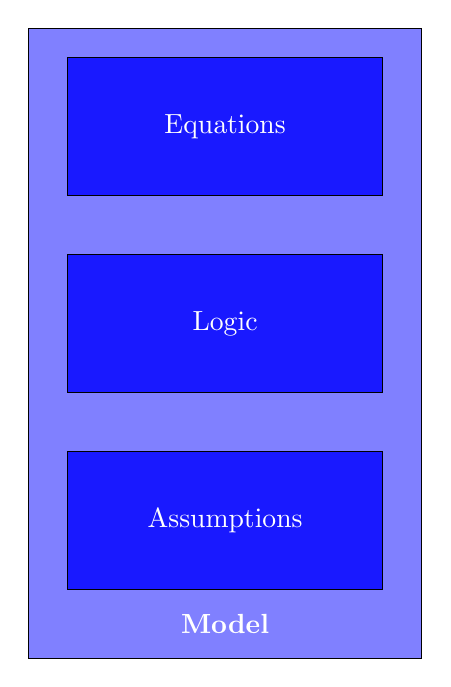
\begin{tikzpicture}
\coordinate [fill=blue!50, minimum width=5cm, minimum height=8cm, rectangle, draw] (c76dabc2-1964-4a10-b72a-88fafa6f2138) at (1.25, 4) {};
\node [text=white, above=0.2cm ] (ab3d5dad-7dfb-43ae-aa5d-3acc752e0aad) at (c76dabc2-1964-4a10-b72a-88fafa6f2138.south) {\textbf{Model}};
\node [fill=blue!90, minimum width=4cm, minimum height=1.75cm, rectangle, draw, text=white] (f9bf7c24-76fd-46b5-aab1-e33305c3d589) at (1.25, 1.75) {Assumptions};
\node [fill=blue!90, minimum width=4cm, minimum height=1.75cm, rectangle, draw, text=white] (77b7cfc5-f237-4b8b-ade6-b2b41b402949) at (1.25, 4.25) {Logic};
\node [fill=blue!90, minimum width=4cm, minimum height=1.75cm, rectangle, draw, text=white] (170050d0-04a2-4a41-8a84-c7c58c1e31e8) at (1.25, 6.75) {Equations};
\end{tikzpicture}
\end{adjustbox}
\end{center}
\end{frame}
\begin{frame}
\frametitle{What Did we Assume?}
\begin{itemize}
\item We made a few assumptions last time in building a general retirement model
\end{itemize}
\vfill
\begin{block}<+>{Assumptions}
\begin{enumerate}
\item The salary is constant over time
\item The savings rate is constant over time
\item Investment returns are constant over time
\item The amount needed in retirement is given by a fixed amount of desired cash
\item The amount needed in retirement does not depend on market conditions or life situations
\end{enumerate}
\end{block}
\end{frame}
\end{section}
\begin{section}[Relax Assumptions]{Extending the Model by Relaxing Assumptions}
\begin{frame}
\frametitle{Relaxing the salary assumption}
\begin{itemize}
\item Assumptions can be relaxed to create a more realistic model
\vfill
\item Often we still need an assumption, but it can be a more realistic one
\vfill
\item We shall relax the constant salary assumption
\vfill
\item \textbf{New assumption: }
The salary grows at a constant rate for cost of living raises, and every number of years the salary grows at an additional rate for a promotion.
\end{itemize}
\end{frame}
\begin{frame}
\frametitle{Relaxing the salary assumption}
\begin{block}{The Equation from the New Assumption}
\begin{center}
\begin{adjustbox}{width=0.9\textwidth, height=0.8\textheight, keepaspectratio}
$S_t = S_0 (1 + r_l)^t (1 + r_p)^p$
\end{adjustbox}
\end{center}
\begin{itemize}
\item $S_t$:  Salary at year $t$
\item $S_0$:  Starting wealth
\item $r_l$:  Return for cost of living
\item $r_p$:  Return for promotion
\item $t$:  Number of years
\item $p$:  Number of promotions
\end{itemize}
\end{block}
\end{frame}
\end{section}
\begin{section}[Advanced Excel]{Advanced Excel Modeling}
\begin{frame}
\frametitle{An Organized Structure of an Advanced Excel Model}
\begin{columns}
\begin{column}{0.5\textwidth}
\vbox to 0.8\textheight{\begin{itemize}
\item We are going to build our first complex Excel model
\vfill
\item It is important to start structuring your model so that it is navigatable
\vfill
\item Inputs in one area, outputs in one area, sub-models in individual tabs
\end{itemize}}
\end{column}
\begin{column}{0.5\textwidth}
\vbox to 0.8\textheight{\centering
\vfill

\includegraphics[height=1.0\textheight, keepaspectratio, width=0.9\textwidth]{Sources/excel-logo.png}
\vfill
\vfill}
\end{column}
\end{columns}
\end{frame}
\begin{frame}
\frametitle{Modeling Salary Growth in Excel - If Command}
\begin{itemize}
\item We need to learn a few formulas and patterns in Excel to model the new assumption
\vfill
\item 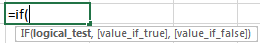
\includegraphics[width=0.5\textwidth]{Sources/excel-if.png}
\vfill
\item \texttt{=IF(5=5, "this", "that")}
-> "this"
\vfill
\item \texttt{=IF(4=5, "this", "that")}
-> "that"
\end{itemize}
\end{frame}
\begin{frame}
\frametitle{Modeling Salary Growth in Excel - Modulo}
\begin{itemize}
\item 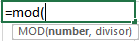
\includegraphics[width=0.3\textwidth]{Sources/excel-mod.png}
\vfill
\item Returns the remainder after a number is divided by a divisor
\vfill
\item \texttt{=MOD(3, 4)}
-> 3
\vfill
\item \texttt{=MOD(7, 2)}
-> 1
\end{itemize}
\end{frame}
\begin{frame}
\frametitle{Modeling Salary Growth in Excel - Table Lookup}
\begin{itemize}
\item 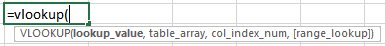
\includegraphics[width=0.5\textwidth]{Sources/excel-vlookup.png}
\vfill
\item Use VLOOKUP when you need to find things in a table or by row
\vfill
\item 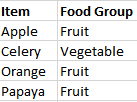
\includegraphics[width=0.2\textwidth]{Sources/excel-vlookup-example-table.png}
\vfill
\item \texttt{=VLOOKUP("Celery", J3:K6, 2)}
-> "Vegetable"
\vfill
\item Lookup column must be first column, and must be sorted in ascending order.
\end{itemize}
\end{frame}
\begin{frame}
\frametitle{Salary Growth in Excel}
{
\setbeamercolor{block title}{bg=darkgreen}
\begin{block}{Extending the Excel Retirement Model for Realistic Salaries}
\begin{itemize}
\item I will now relax the assumption that salary is a fixed number in the Excel model.
\item As this will be quite different from the last model, I will start from scratch.
\item I have uploaded the finished product to Examples > Intro > Excel > "Dynamic Salary Retirement Model.xlsx"
\end{itemize}
\end{block}
}
\end{frame}
\begin{frame}
\frametitle{Relaxing the Static Desired Cash in Excel}
\begin{itemize}
\item We want to relax the assumption that the amount needed in retirement is given by a fixed amount of desired cash
\end{itemize}
\vfill
{
\setbeamercolor{block title}{bg=violet}
\begin{block}{Modeling Desired Cash}
\begin{itemize}
\item Add new inputs to the model, "Annual Cash Spend During Retirement" and "Years in Retirement"
\item Calculate desired cash based on interest, cash spend, and years in retirement
\item Use the calculated desired cash in the model to determine years to retirement
\item If annual spend is 40k for 25 years in retirement, \$563,757.78 should be the retirement cash
\end{itemize}
\vfill
\end{block}
}
\end{frame}
\end{section}
\end{document}